\subsection{Lie Groups and Their algebra}
对于一个李群,定义其在单位元处的切空间为其李代数:
\[g:=T_1G\]
关于李群有相关的映射及其诱导的切空间之间的映射,如图\ref{fig:basicmap} 所示。
\begin{figure}
\begin{center}
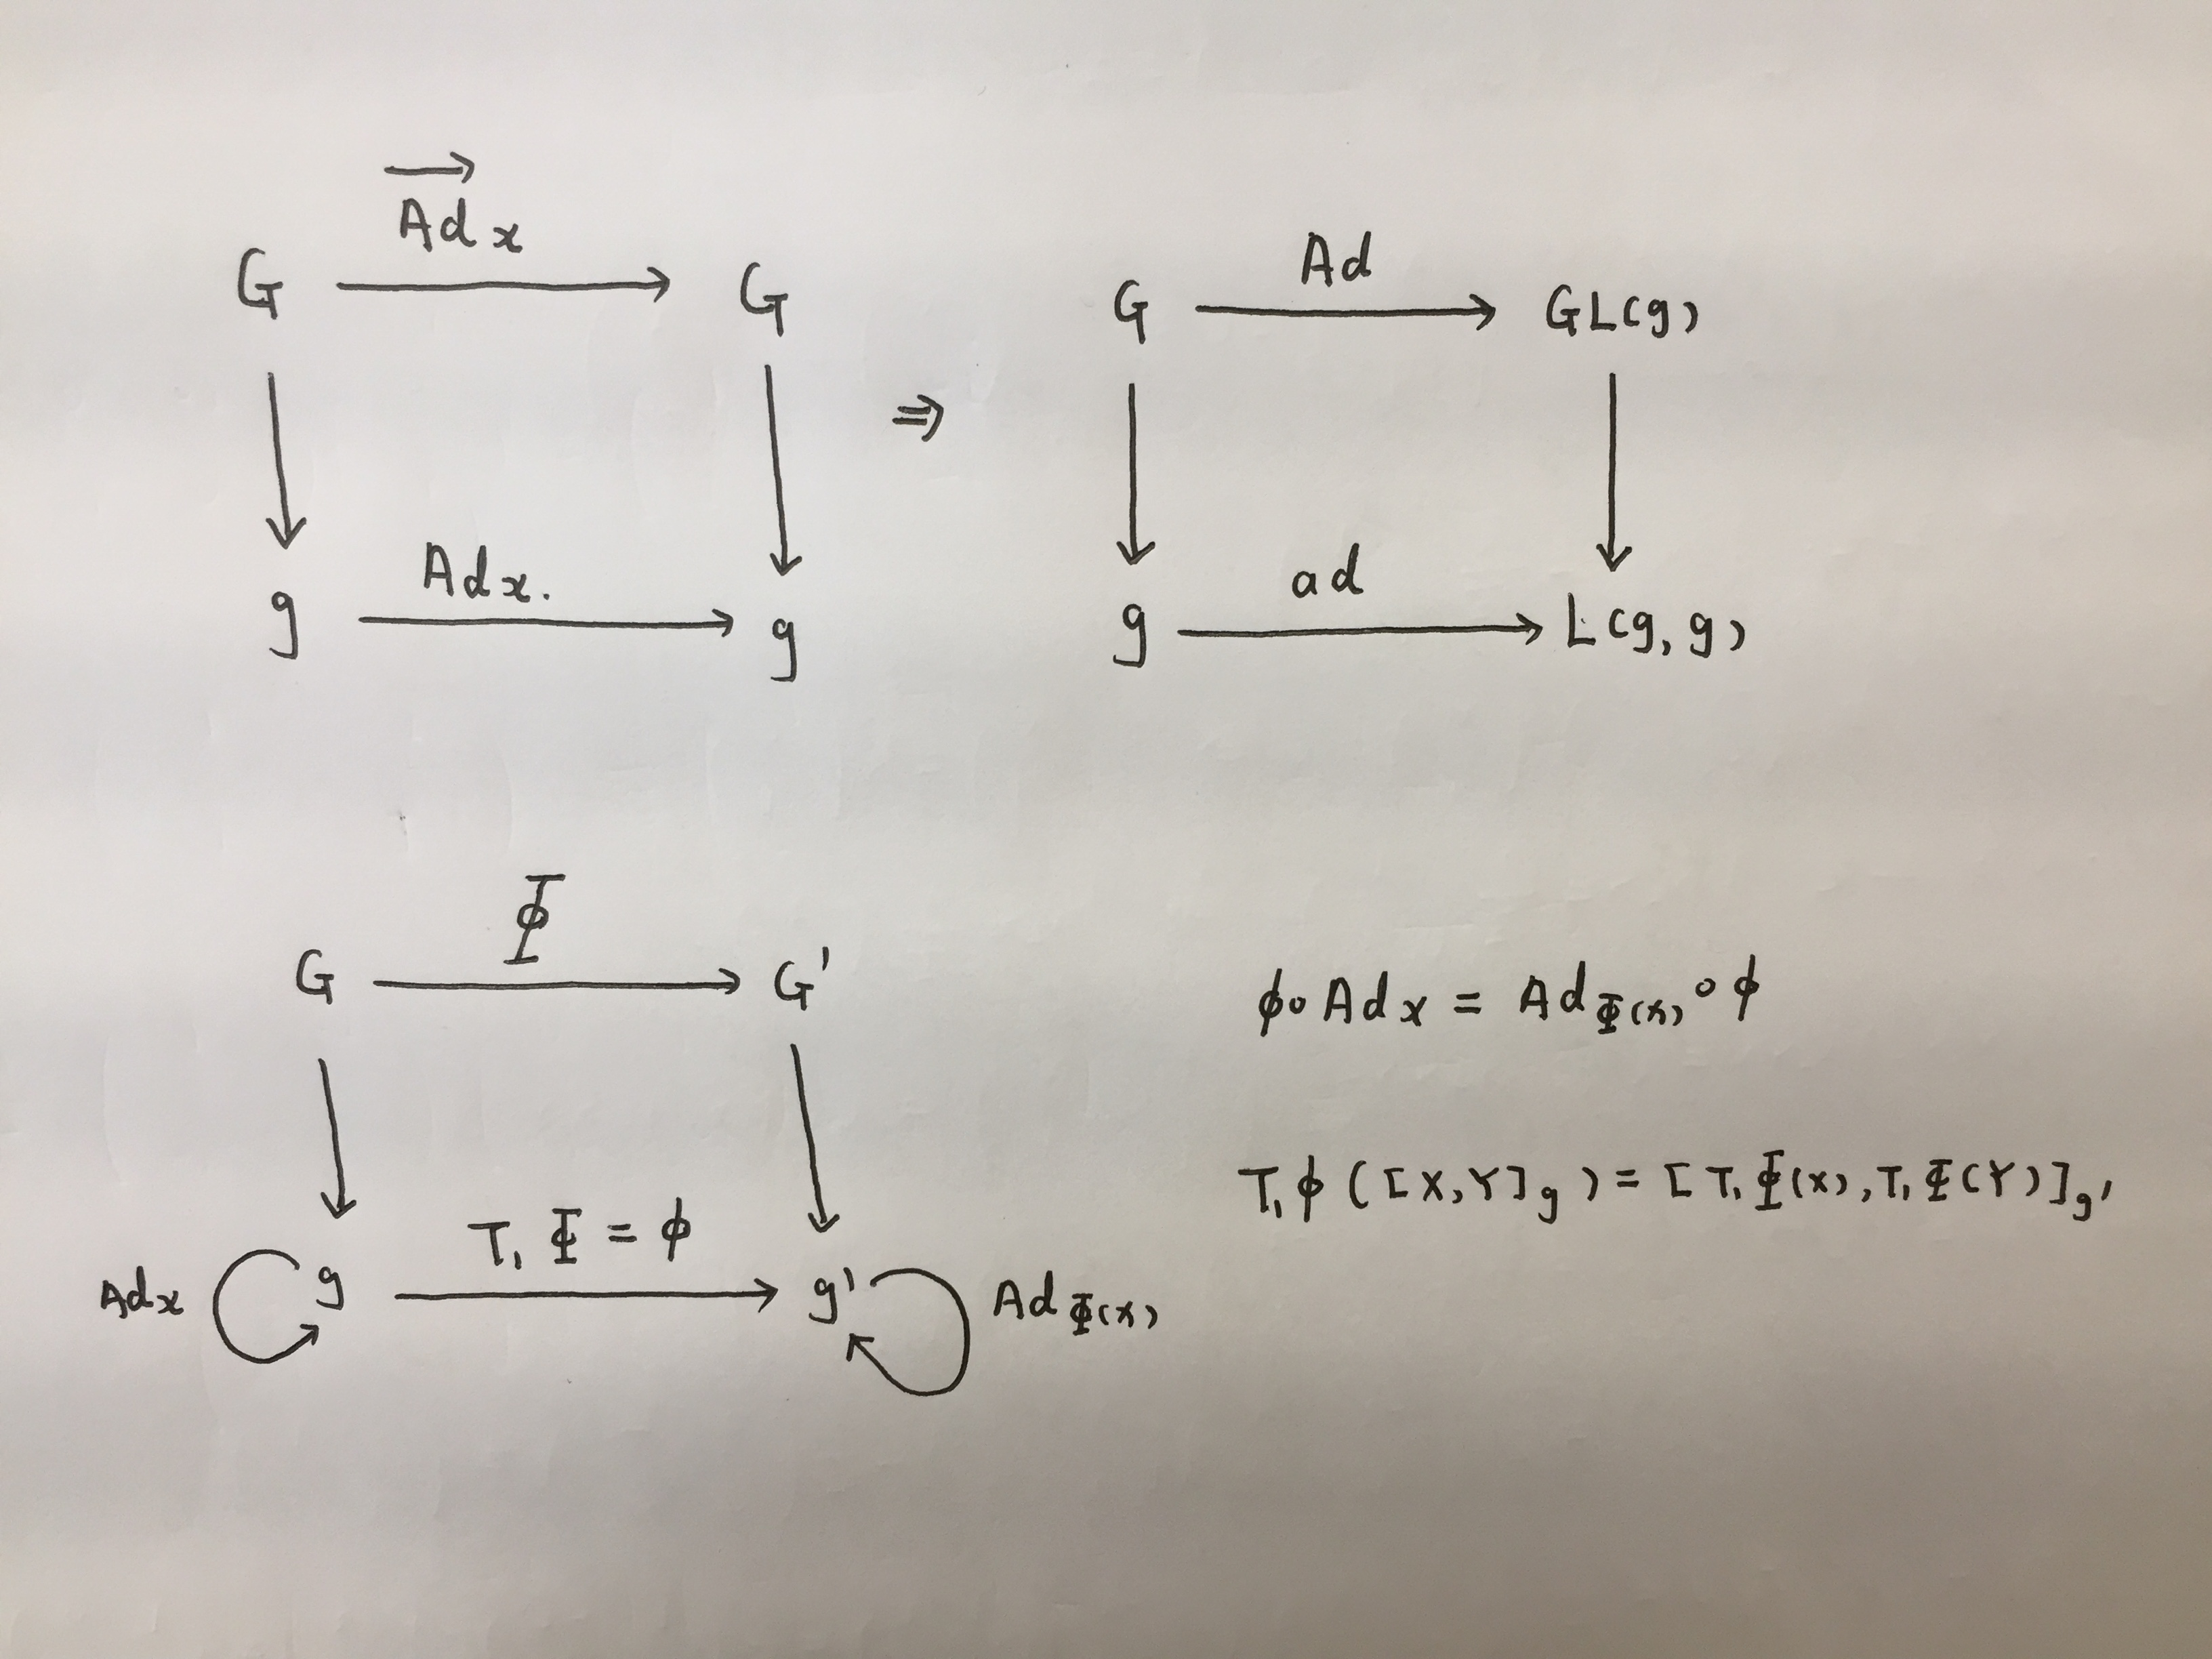
\includegraphics[height=8cm]{figures/Mappings.JPG}
\caption{李群之间的基本映射}
\label{fig:basicmap}
\end{center}
\end{figure}
其中我们有:
\[ad(X)(Y)=[X,Y]\]
李括号之间的基本性质:
\[[X,[Y,Z]]+[Y,[Z,X]]+[Z,[X,Y]]=0\]
常见的李群之正交群
\[O(n,R)=\{A\in L(R^n,R^n)|A^TA=I\}\]
它的李代数为:
\[o(n,R)=\{X\in L(R^n,R^n)|X^T+X=0\}\]
特殊正交群:
\[SO(n,R)=\{A\in O(n,R)|det(A)=1\}\]
它的李代数为:
\[so(n,R)=\{X\in L(R^n,R^n)|X^T+X=0 tr(X)=0\}\]
对于SO(3,R)中的元素,可以表示为:
\[R_x=I+\frac{sin|x|}{|x|}A_x+\frac{1-cos|x|}{|x|^2}A_x^2\]
其中x为$R^3$中的元素且:
\begin{equation}
A_x=\left(\begin{array}{ccc}
0&-x_3&x_2\\
x_3&0&-x_1\\
-x_2&x_1&0\\
\end{array}
\right)
\end{equation}

也就是说,这给出了从$R^3$到SO(3,R)中的元素的一个映射。\par
SO(3,R)中的共轭类为:
\[C_c=\{R_x|x\in R^3,|x|=c\}\]
且他的基本群为:
\[\pi_1(SO(3,R))=Z/2Z\]
Unitary Group:
\[U(n)=\{A\in L_C(C^n,C^n)|A^\dagger A=I\}\]
它的李代数为:
\[u(n)=\{A\in L_C(C^n,C^n)|A^\dagger+A=0\}\]
Special Unitary Group:
\[SU(n)=\{A\in U(n)|det(A)=1\}\]
它的李代数为:
\[su(n)=\{A\in u(n)|tr(A)=0\}\]
对于SU(2),我们有:
\[SU(2)=\{\left(\begin{array}{cc}a&b\\-\bar{b}&\bar{a}\\\end{array}\right)|a,b\in C,|a|^2+|b|^2=1\}\]
SU(2)的共轭类为:
\[C_c=\{A\in SU(2)|Re(a)=c\}\]
对于SU(2)的李代数,我们有:
\[su(2)=\{\left(\begin{array}{cc}i\alpha&\beta\\-\bar{\beta}&-i\alpha\\\end{array}\right)|\alpha\in R,\beta\in C\]
special linear group:
\[SL(n,R)=\{A\in L_R(R^n,R^n)|det(A)=1\}\]
它的李代数为:
\[sl(n,R)=\{A\in L_R(R^n,R^n)|tr(A)=0\}\]

\subsection{The Exponential Map}
左右平移算符:
\[R(x)y=yx\]
\[L(x)y=xy\]
对于左右平移算符,我们有:
\[R(x)L(y)=L(y)R(x)\]
\[L(xy)=L(x)L(y)\]
\[R(xy)=R(y)R(x)\]
对于流形上的左不变向量场v,我们定义为:
\[v_{L(x)y}=T_yL(x)v_y\]
对于流形上的右不变向量场v,我们定义为:
\[v_{R(x)y}=T_yR(x)v_y\]
流形上的左右不变向量场记为:
\[X^L,X^R\]
\begin{lemma}
Let $\Phi^t$ be a  the flow of a left or' right invariant vector field v on G.this is a $C^2$ mapping G$\rightarrow$ G satisfying:\par
\begin{center}
\begin{tabular}{cc}
$\Phi^t=R(\Phi^t(1))$&if v is left invariant\\
$\Phi^t=L(\Phi^t(1))$&if v is right invariant\\
\end{tabular}
\end{center}
\end{lemma}

\begin{theorem}
For Every $X\in g$ there is a unique homomorphism $h=h_X$:(R,+)$\rightarrow (G,\cdot)$ that is differentiable at t = 0 and satisfies $\frac{dh}{dt}(0)=X$ It is equal to the solution curve of both $X^L$ and of $X^R$ starting at the identity element of G. The flows of $X^L$ and of $X^R$ are globally defined for all $t \in R$
\end{theorem}
so with this theorem,we can define the exponetial map form g to G which yield as:
\[Exp(X)=h_X(1)\]
one can easily get that:
\[h_X(st)=h_{tX}(s)\]
then set s=1 one can get:
\[h_X(t)=exp(tX)\]

differential the above function with respect to t one can get:
\begin{center}
\begin{tabular}{cc}
$X=T_0(exp)(X)$&for any X$\in$ g\\
\end{tabular}
\end{center}
so $T_0(exp)$ is equal to the identity,and  the $C^1$ diffeomorphism from U onto V opposite to exp is called log.\par
\subsection{The exponetial map of vector space}
we can define :
\[e^A=\sum_k\frac{1}{k!}A^k\]
we set $A(t)=e^{tX}$ then:
\[\frac{dA(t)}{dt}=XA(t)=T_1R(A(t))(X)=X^R(A(t))\]
so A(t) is a flow of X which imply that:
\[exp(X)=A(1)=e^X\]
one can easily get the relation:
\[det(e^A)=e^{tr(A)}\]
\subsection{the tanget map of Exp}
\begin{lemma}
Let G, and H, be Lie groups, with Lie algebra equal to g, and h, respectively. Suppose that if> is a homomorphism: G $\rightarrow$ H that is differentiable at 1 $\in$ G. Then$\Phi(expX) = exp(T_1\Phi(X))$, for each $X\in g$.
\end{lemma}
\begin{theorem}
\[Ad(exp(X))=e^{ad(X)}\]
\[xe^Xx^{-1}=e^{(Ad_x)(X)}\]
\end{theorem}

\begin{theorem}
For any $X\in g$  the linear mapping $T_Xexp:g\rightarrow T_{exp(X)}G$ is given by:
\[T_Xexp=T_1R(exp(X))\circ \int_0^1e^{sadX}ds=T_1L(exp(X))\circ\int_0^1e^{-s adX}ds\]
\end{theorem}
which is illustrated in figure\ref{fig:TxExp1} and figure\ref{fig:TxExp2}\par
\begin{figure}
\begin{minipage}[t]{0.5\linewidth}
\centering
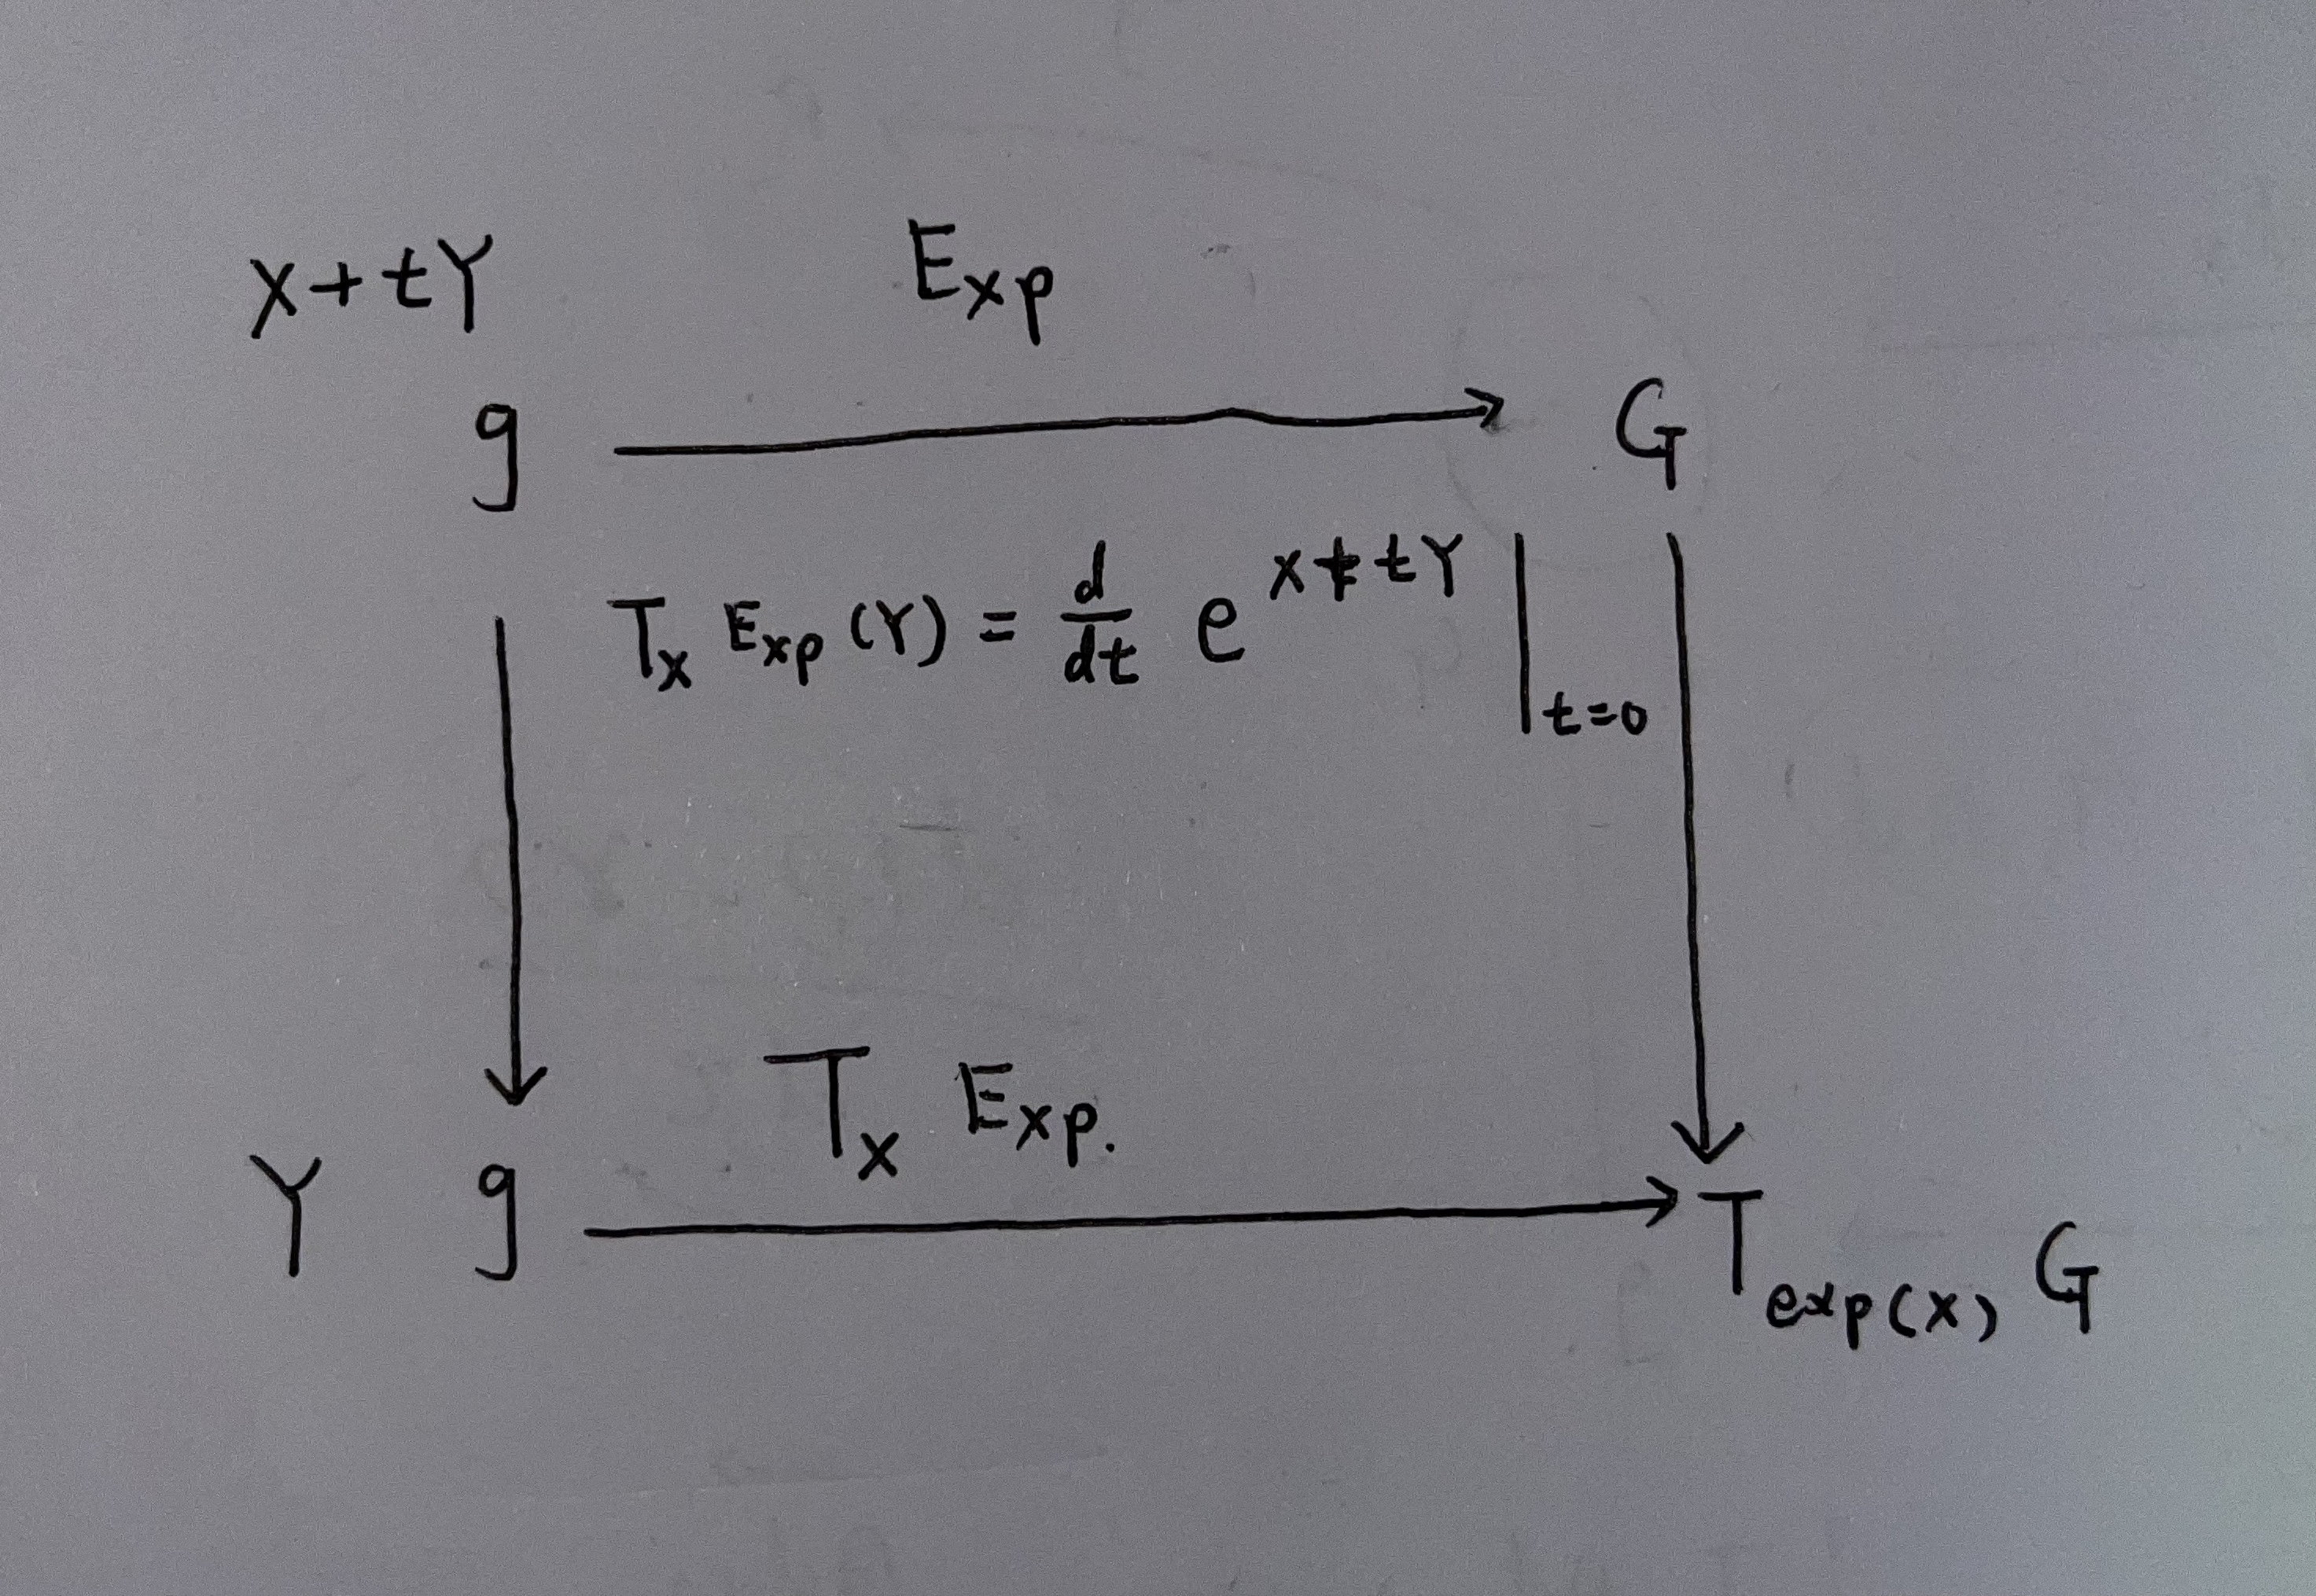
\includegraphics[width=\textwidth,height=6cm]{figures/TxExp1.jpg}
\caption{}
\label{fig:TxExp1}
\end{minipage}
\begin{minipage}[t]{0.5\linewidth}
\centering
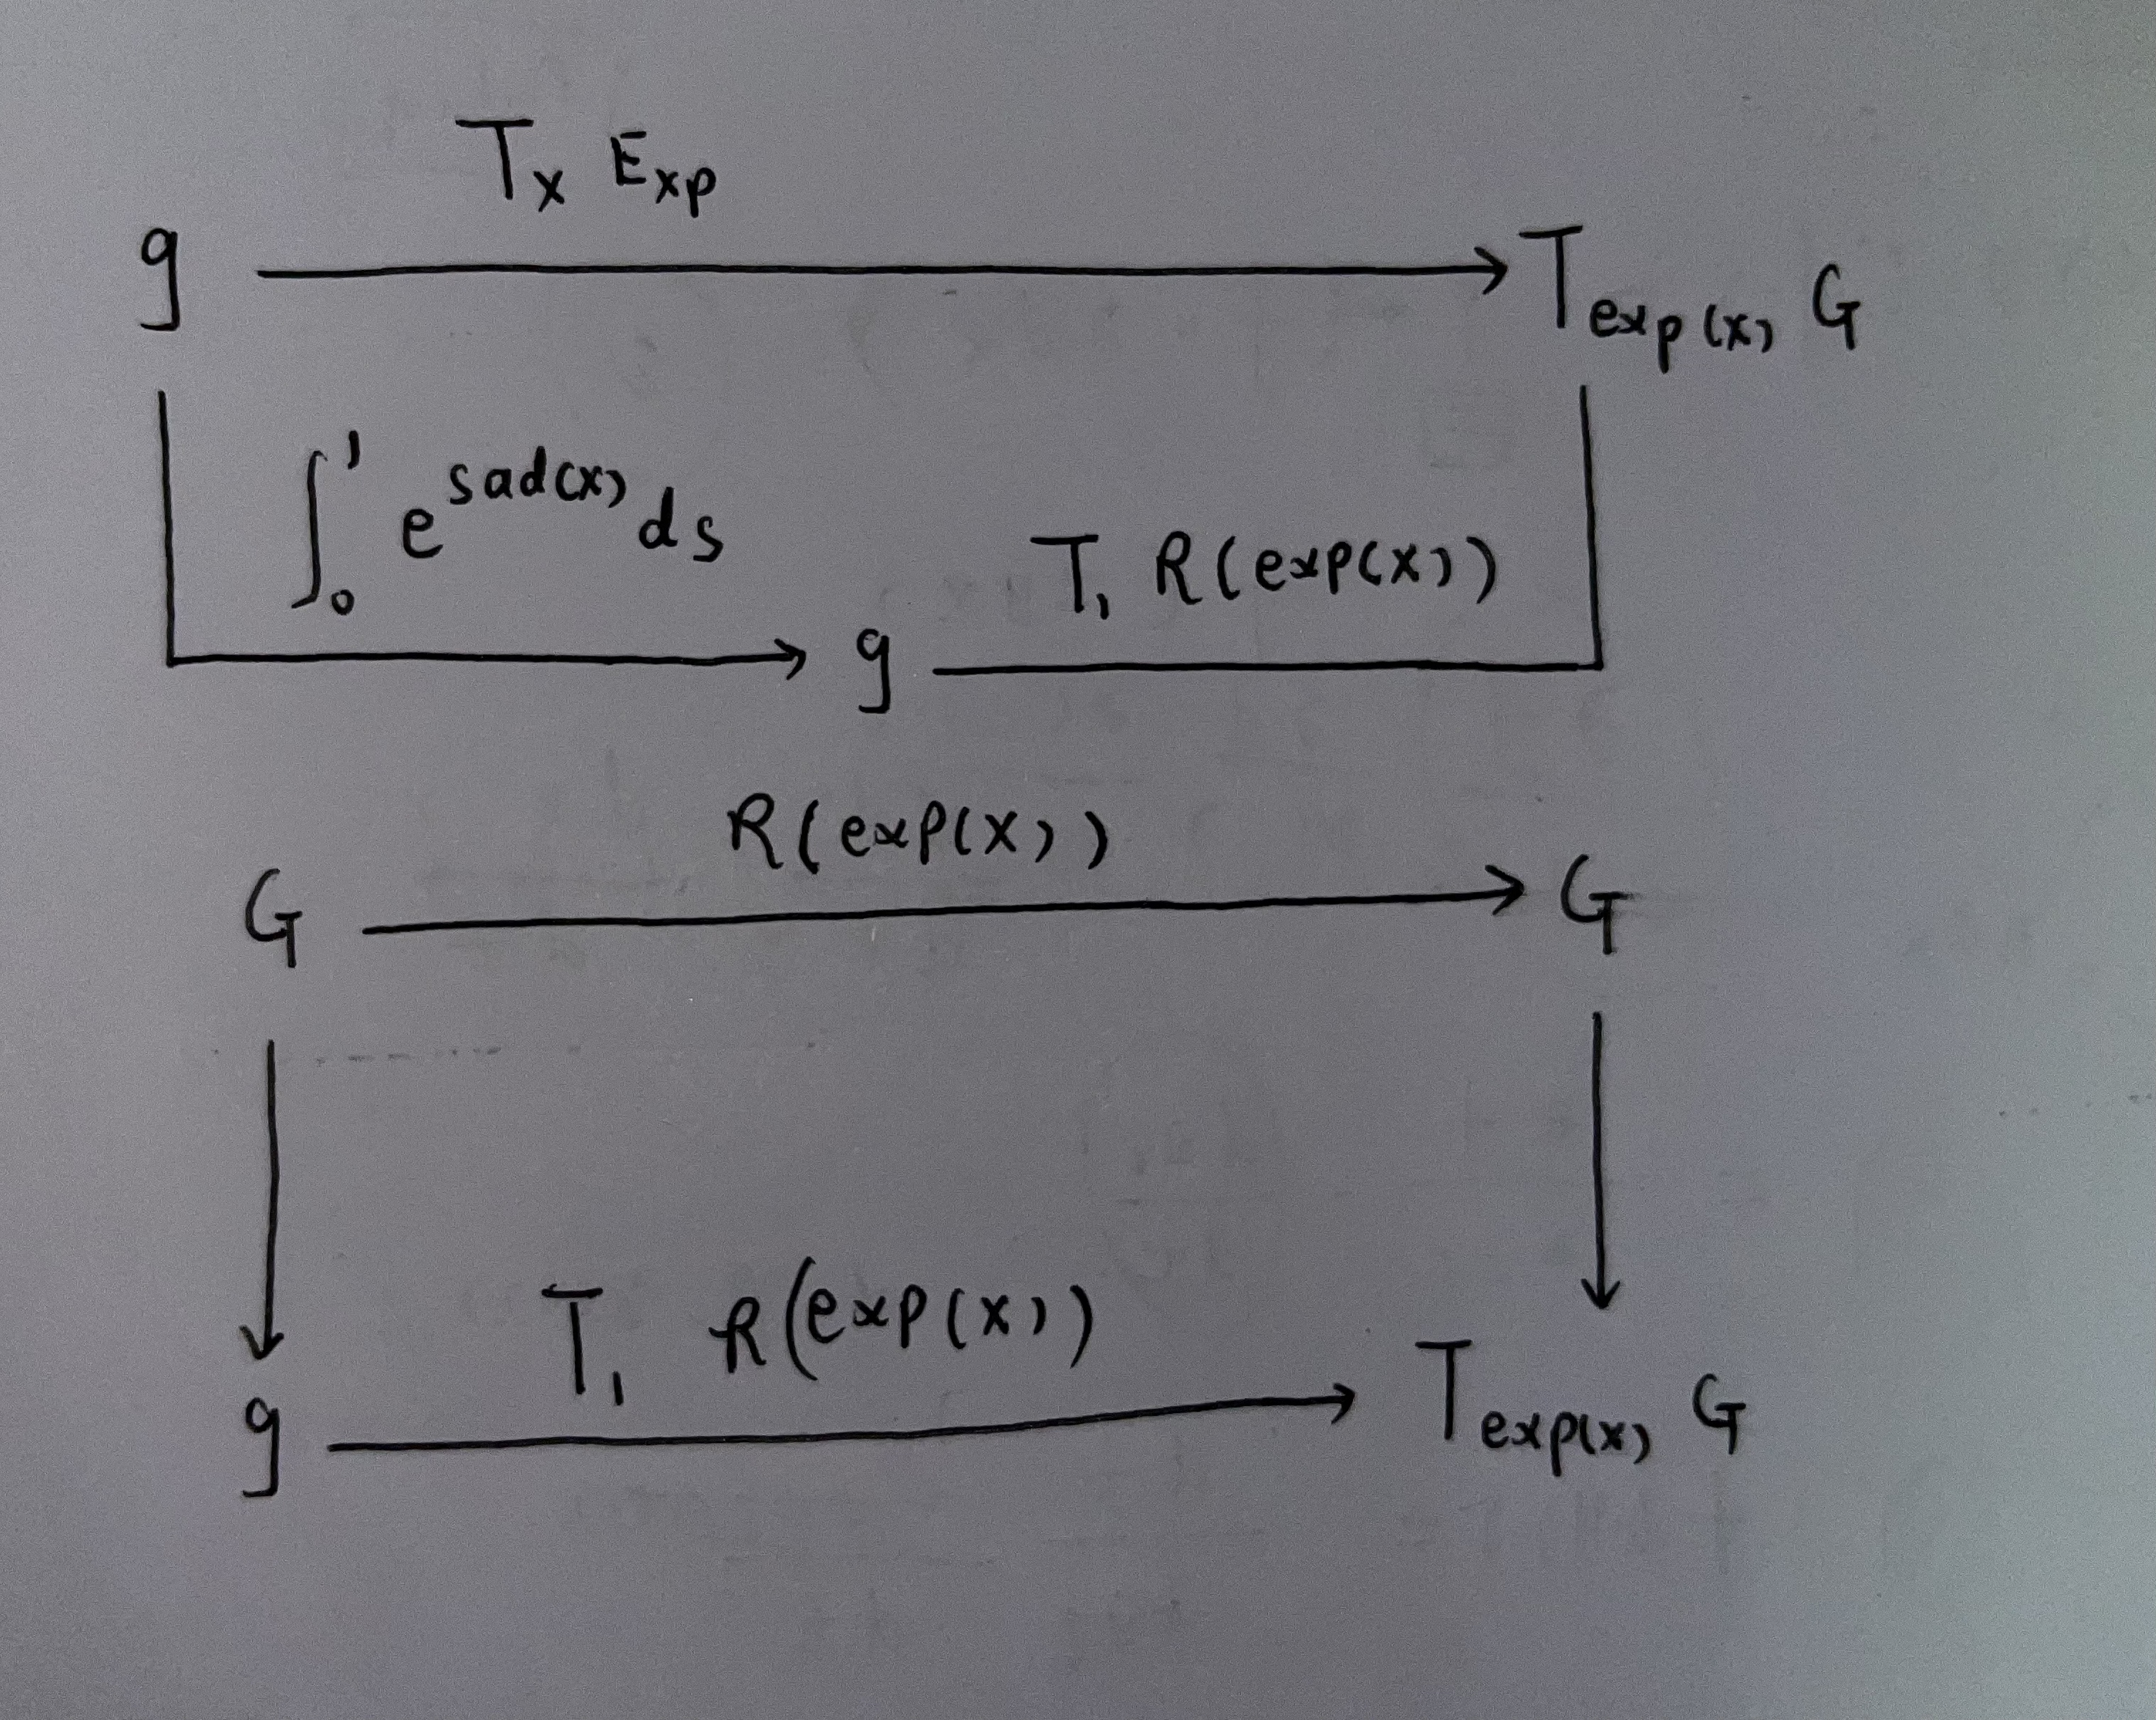
\includegraphics[width=\textwidth,height=6cm]{figures/TxExp2.jpg}
\caption{}
\label{fig:TxExp2}
\end{minipage}
\end{figure}

we can define a function of A as:
\[f(A):=\int_0^1e^{sA}ds=A^{-1}(e^A-I)\]
if A is invertible,then we have the corresponding definnition and if A is not invertible we define:
\[A^{-1}(e^A-I):=\int_0^1e^{sA}ds\]
\begin{lemma}
The singular points of the exponential mapping: $g \rightarrow G$, that is, the $X \in g$ such that $T_X$exp is not invertible, are precisely the $X \in g$ such that $ad X \in L(g, g)$ has an eigenvalue of the form $2\pi ik$, with $k \in Z \{O\}$
\end{lemma}
we can define the sets:
\[\Sigma_1:=\{X\in g| det(ad(X)-2\pi ik)=0\}\]
\subsection{The Product in Logarithmic Coordinates}
define a map from R to g which is:
\[t\in R \rightarrow (Z(t))\in g\]
that Z(t) satisfying the equation:
\[\frac{dZ(t)}{dt}=\frac{ad Z(t)}{e^{ad Z(t)}-I}(X), Z(0)=Y\]
set $g_e^2$ be the set of $(X,Y)\in(g,g_e)$ such the above solution is defined for all $t\in [0,1]$,make:
\[\mu(X,Y)=Z(1)\]
then we have the below theorem:
\begin{theorem}the set $g_e^2$ is an open neighborhood of (0, 0) in (g,g) and $\mu$ is a real-analytic mapping $g_e^2\rightarrow g$ .If g is the Lie algebra of a Lie group G, with exponential mapping exp then:
\[exp(X)exp(Y)=exp(\mu(X,Y))\]
\end{theorem}
 the mapping $\mu(X,Y)$ is called \textcolor{blue}{the product in logarithmic coordinates.}\par
pick up a open neigborhood of g in 0 $U_0$ then for the map:
\[V_0^x=L(x)exp(U_0)\]
\[k^x(y)=\ln(x^{-1}y)\]
we have the following theorem:
\begin{theorem}
The $k^x: V_0^x\rightarrow U_0$, for $x \in G$, form a real-analytic atlas for G, making G into a real-analytic Lie group $G_{an}$ , such that the identity in G is a $C^2$ diffeomorphism between G and $G_{an}$ . Furthermore, if g is a complex Lie algebra , then this atlas is complex-analytic. It makes G into a complex-analytic group if in addition $Ad_x$ is complex-linear: $g \rightarrow g$, for every $x \in G$.
\end{theorem}
\subsection{Dynkin's Formula}
\[\mu(X,Y)=X+Y+\sum_{k=1}^\infty\frac{(-1)^k}{k+1}\sum_{l_1\cdots l_k,m_1\cdots m_k\geq 0 ,l_i+m_i>0}\frac{1}{l_1+l_2+\cdots l_k}(\frac{(ad X)^{l_1}}{l_1!}\frac{(ad Y)^{m_1}}{m_1!}\cdots\frac{(ad X)^{l_k}}{l_k!}\frac{(ad Y)^{m_k}}{m_k!})(X)\]
so if $[X,[X,Y]]=0$ and $[Y,[X,Y]]=0$ then,we have:
\[\mu(X,Y)=X+Y+\frac{1}{2}[X,Y]\]
then we have:
\[e^Xe^Y=e^{X+Y+\frac{1}{2}[X,Y]}\rightarrow e^{X+Y}=e^Xe^Ye^{-\frac{1}{2}[X,Y]}\]

